\documentclass{article}
\usepackage{gvv-book}
\usepackage{gvv}
\usepackage{amsmath}
\usepackage{amsfonts}
\usepackage{tikz}
\usepackage{setspace}
\usepackage{gensymb}
\usepackage[cmex10]{amsmath}
\usepackage{amsthm}
\usepackage{mathrsfs}
\usepackage{txfonts}
\usepackage{stfloats}
\usepackage{bm}
\usepackage{cite}
\usepackage{cases}
\usepackage{subfig}
\usepackage{longtable}
\usepackage{multirow}
\usepackage{enumitem}
\usepackage{mathtools}
\usepackage{tikz}
\usepackage{circuitikz}
\usepackage{verbatim}
\usepackage[breaklinks=true]{hyperref}
\usepackage{tkz-euclide}
\usepackage{listings}
\usepackage{color}    
\usepackage{array}    
\usepackage{longtable}
\usepackage{calc}     
\usepackage{multirow} 
\usepackage{hhline}   
\usepackage{ifthen}   
\usepackage{lscape}     
\usepackage{chngcntr}
\usepackage{graphicx}
\usepackage{float}
\usepackage{multicol}
\usepackage[a4paper, left = 1.5cm, right = 1.5cm]{geometry}

\begin{document}

\begin{center}
\large
    \textbf{Samyak Gondane-AI25BTECH11029}
\end{center}
\date{}

\section*{Question}
Draw a triangle $ABC$ with $BC = 7\ cm$, $\angle B = 45\degree$ and $\angle C = 60\degree$.

\section*{Solution}


\subsection*{Given}
\begin{itemize}
    \item $BC = a = 7\ cm$
    \item $\angle B = 45\degree$
    \item $\angle C = 60\degree$
\end{itemize}
\\
Let $\vec{B}$ be the origin

\begin{align}
\angle A = 180\degree - (45\degree + 60\degree) = 75\degree
\end{align}




Let:


\begin{align}
\vec{B} = \myvec{0 \\ 0}, \quad
\vec{C} = \myvec{a \\ 0} = \myvec{7 \\ 0}
\end{align}



Direction of $\vec{A}$ is along angle $B = 45\degree$:


\begin{align}
\vec{A} = c \myvec{\cos B \\ \sin B}
= c \frac{1}{\sqrt{2}} \myvec{1 \\ 1}
\end{align}

in $\triangle ABC$
\begin{align}
    b \cos \angle C + c \cos \angle B = 7\\
    b \sin \angle C - c \sin \angle B = 0
\end{align}

Solving linear Equation in b and c:
\begin{align}
    \myvec{\cos \angle C && \cos \angle B \\
    \sin \angle C && -\sin \angle B} \myvec{b \\ c} = \myvec{7 \\ 0}
\end{align}

Using augmented matrix
\begin{align}
    \myvec{\cos \angle C && \cos \angle B &\vrule &7 \\
    \sin \angle C && -\sin \angle B &\vrule &0}
\end{align}

putting $\angle C = 60 \degree$ and $\angle B = 45 \degree$
\begin{align}
    \myvec{1/2 && 1/\sqrt{2} &\vrule &7 \\
    \sqrt{3}/2 && -1/\sqrt{2} &\vrule &0}
\end{align}

Echelon form of the matrix is given by
\begin{align}
    \myvec{1 && 2/\sqrt{2} &\vrule &14 \\
    \sqrt{3}/2 && -1/\sqrt{2} &\vrule &0}
\end{align}

\begin{align}
    \myvec{1 && 2/\sqrt{2} &\vrule &14 \\
    0 && (-1 + \sqrt{3})/\sqrt{2} &\vrule &-7\sqrt{3}}
\end{align}

\begin{align}
    \frac{(- 1 + \sqrt{3})}{\sqrt{2}} \times c = - 7 \sqrt{3}
\end{align}

\begin{align}
    c = \frac{-7\sqrt{3} \cdot \sqrt{2}}{-1 + \sqrt{3}} = \frac{-7\sqrt{6}}{-1 + \sqrt{3}}
\end{align}

\begin{align}
\vec{A} = c \myvec{\cos \angle B \\ \sin \angle B} = -23.42 \myvec{0.7071 \\ 0.7071} \approx \myvec{-16.56 \\ -16.56}
\end{align}

\subsection*{Final Coordinates}


\begin{align}
\vec{A} = \myvec{-16.56 \\ -16.56}, \quad
\vec{B} = \myvec{0 \\ 0}, \quad
\vec{C} = \myvec{7 \\ 0}
\end{align}


\begin{figure}[H]
    \centering
    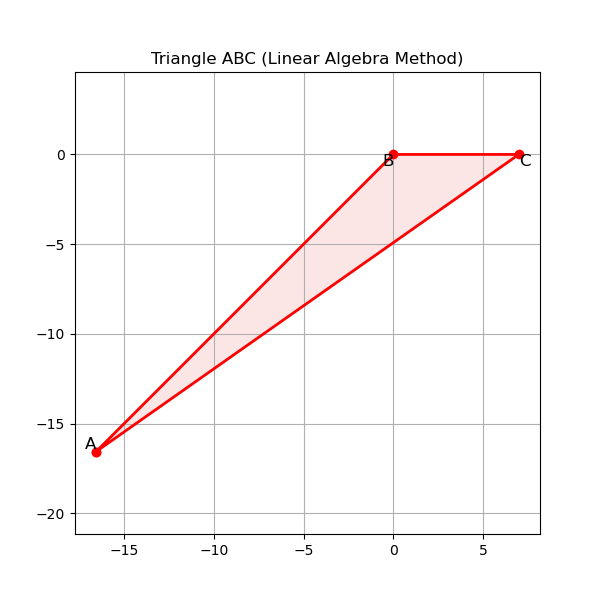
\includegraphics[width=0.7\linewidth]{./figs/Figure_1.png}
    \caption{}
    \label{fig:fig1}
\end{figure}



\end{document}
